%===================================================================%
\section{Vu d'ensemble du projet}
%===================================================================%
% ce qu'on veut permettre
API Catalog est une application web permettant de parcourir les APIs publiées sur une instance WSO2 API Manager, d'afficher leur documentation et de la régénérer automatiquement de manière régulière. Son usage est destiné aux informaticiens du SGSI, des utilisateurs et/ou consultants externes de l'UCLouvain qui souhaitent consulter les APIs publiées sur l'instance API Manager du SGSI afin de faire savoir leur intérêt d'avoir accès à des APIs particulières.\bigskip

% fonctionnalités utilisateurs
Les utilisateurs du catalogue peuvent parcourir les APIs disponibles sur l'instance, les filtrer, les trier, les consulter et télécharger leur documentation.
% ce que ça fait (fonctionnalités)
% elle offre bcp de contrôle aux administrateurs (fontionnalités de gestion)
Cette application offre également aux administrateurs différentes fonctionnalités afin de faciliter sa gestion, notamment :
\begin{itemize}
    \item[$\bullet$] Les données peuvent être rafraîchies manuellement
    \item[$\bullet$] Les APIs peuvent être blacklistées afin de les exclure des rafraîchissements de données
    \item[$\bullet$] Le rythme de rafraîchissement automatique peut être configuré par l'administrateur
\end{itemize}
et tout cela sans avoir à redéployer l'application.\bigskip

% comment c'est fait (Docker Compose, Scheduler, API Manager et apictl) au niveau des technologies elles-mêmes
Le catalogue est déployée en conteneurs via Docker Compose et est constituée de quatre services :
\begin{itemize}
    \item[$\bullet$] \textbf{backend} : une application \href{https://fastapi.tiangolo.com/}{FastAPI} recevant des requêtes afin d'importer les APIs publiées sur l'API Manager (via l'outil en ligne de commande fourni par WSO2 : \href{https://apim.docs.wso2.com/en/latest/reference/apictl/wso2-api-controller/}{APICTL}) et de les extraire dans un répertoire de données partagé.
    \item[$\bullet$] \textbf{frontend} : une application \href{https://flask.palletsprojects.com/en/stable/}{Flask} chargée d'afficher le catalogue et la documentation de chaque API à partir du répertoire de données partagé.
    \item[$\bullet$] \textbf{scheduler} : un lanceur de tâches automatique \href{https://github.com/aptible/supercronic}{Supercronic} lançant automatique le rafraîchissement automatique en appelant le backend à horaire régulier.
    \item[$\bullet$] \textbf{proxy} : un proxy \href{https://nginx.org/}{Nginx} pour le frontend et le backend permettant d'exposer les services en HTTPS.
\end{itemize}
\bigskip

Dans ce document nous irons plus en détail dans l'architecture, la structure, le fonctionnement et les limitations de l'application. Nous terminerons par des points d'amélioration et une conclusion.
%%%%%%%%%%%%%%%%%%%%%%%%%%%%%%%%%%%%%%%%%%%%%%%%%%%%%%%%%%%%%%%%%%%%%
%                                                                   %
%                                                                   %
%                                                                   %
%                                                                   %
%                                                                   %
%                                                                   %
%                                                                   %
%                                                                   %
%===================================================================%
\newpage
\section{Diagramme d'architecture}
%===================================================================%
API Catalog suit la structure suivante :
\begin{figure}[H]
    \centering
    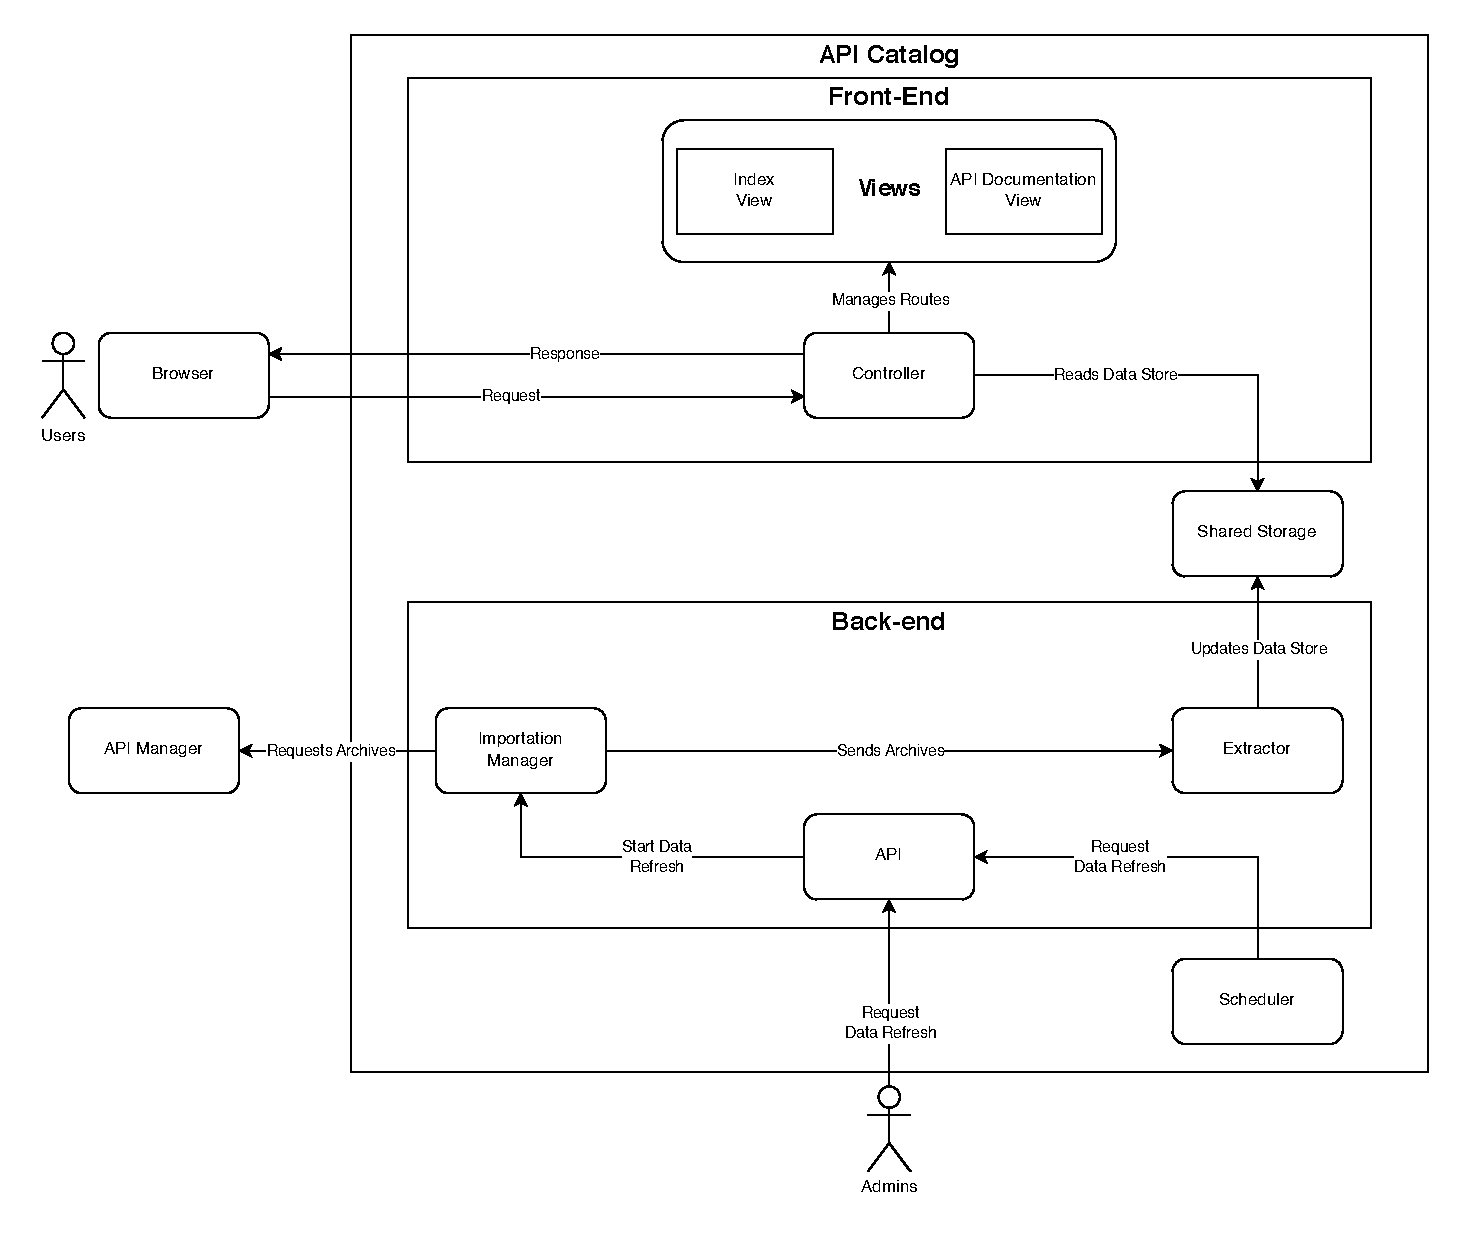
\includegraphics[width=1.\textwidth]{img/architecture_diagram.pdf}
    \caption{Diagramme d'architecture}
\end{figure}
\bigskip

Les trois services \textbf{backend}, \textbf{frontend} et \textbf{scheduler} communiquent ensemble via le réseau interne de Docker (\texttt{bridge}) et ne sont pas exposés à l'extérieur sauf par l'hôte qui a également accès à ce réseau.
%%%%%%%%%%%%%%%%%%%%%%%%%%%%%%%%%%%%%%%%%%%%%%%%%%%%%%%%%%%%%%%%%%%%%
%                                                                   %
%                                                                   %
%                                                                   %
%                                                                   %
%                                                                   %
%                                                                   %
%                                                                   %
%                                                                   %
%===================================================================%
\newpage
\section{Structure du projet}
%===================================================================%
\begin{lstlisting}[caption={Structure du projet}]
apictl/
    apictl
    login.sh
    keys.json.example
    ...
backend/
    api_archive_extractor.py
    apictl_client.py
    api_manager_client_interface.py
    backend.py
    blacklist.txt
    importation_manager.py
    utils.py
    ...
data/
docker/
    Dockerfile.backend
    Dockerfile.frontend
    Dockerfile.scheduler
frontend/
    static/
        font/...
        icon/...
        redoc/
            redoc.standalone.js
            ...
        filter.js
        style.css
    templates/
        403.html
        404.html
        415.html
        base.html
        card.html
        contact.html
        documentation.html
        footer.html
        index.html
        navbar.html
        redoc.html
        viewer.html
    api_metadata_extractor.py
    frontend.py
    ...
proxy/
    deploy/
        certs/...
        proxy.conf
    snakeoil.sh
scheduler/crontab
compose.yaml
compose.proxy.yaml
.editorconfig
.env.example
...
\end{lstlisting}
\bigskip





%%%%%%%%%%%%%%%%%%%%%%%%%%%%%%%%%%%%%%%%%%%%%%%%%%%%%%%%%%%%%%%%%%%%%
%                                                                   %
%                                                                   %
%                                                                   %
%                                                                   %
%                                                                   %
%                                                                   %
%                                                                   %
%                                                                   %
%===================================================================%
\section{Service backend}
%===================================================================%
Le backend FastAPI peut recevoir des requêtes HTTP afin de lancer le processus de rafraîchissement des données à la requête de l'administrateur via l'hôte ou automatiquement depuis le scheduler via le réseau interne de Docker (\verb|bridge|).



%%%%%%%%%%%%%%%%%%%%%%%%%%%%%%%%%%%%%%%%%%%%%%%%%%%%%%%%%%%%%%%%%%%%%
%                                                                   %
%                                                                   %
%                                                                   %
%                                                                   %
%                                                                   %
%                                                                   %
%                                                                   %
%                                                                   %
%===================================================================%
\section{Service frontend}
%===================================================================%



%%%%%%%%%%%%%%%%%%%%%%%%%%%%%%%%%%%%%%%%%%%%%%%%%%%%%%%%%%%%%%%%%%%%%
%                                                                   %
%                                                                   %
%                                                                   %
%                                                                   %
%                                                                   %
%                                                                   %
%                                                                   %
%                                                                   %
%===================================================================%
\section{Service scheduler}
%===================================================================%



%%%%%%%%%%%%%%%%%%%%%%%%%%%%%%%%%%%%%%%%%%%%%%%%%%%%%%%%%%%%%%%%%%%%%
%                                                                   %
%                                                                   %
%                                                                   %
%                                                                   %
%                                                                   %
%                                                                   %
%                                                                   %
%                                                                   %
%===================================================================%
\section{Service proxy}
%===================================================================%



%%%%%%%%%%%%%%%%%%%%%%%%%%%%%%%%%%%%%%%%%%%%%%%%%%%%%%%%%%%%%%%%%%%%%
%                                                                   %
%                                                                   %
%                                                                   %
%                                                                   %
%                                                                   %
%                                                                   %
%                                                                   %
%                                                                   %
%===================================================================%
\section{Limitations}
%===================================================================%
\subsection{Style du Frontend}
% pas de bootstrap à cause du Redoc



%%%%%%%%%%%%%%%%%%%%%%%%%%%%%%%%%%%%%%%%%%%%%%%%%%%%%%%%%%%%%%%%%%%%%
%                                                                   %
%                                                                   %
%                                                                   %
%                                                                   %
%                                                                   %
%                                                                   %
%                                                                   %
%                                                                   %
%===================================================================%
\section{Points d'amélioration}
%===================================================================%
% cfr TODO.md



%%%%%%%%%%%%%%%%%%%%%%%%%%%%%%%%%%%%%%%%%%%%%%%%%%%%%%%%%%%%%%%%%%%%%
%                                                                   %
%                                                                   %
%                                                                   %
%                                                                   %
%                                                                   %
%                                                                   %
%                                                                   %
%                                                                   %
%===================================================================%
\section{Conclusion}
%===================================================================%
% ça marche, ça rempli les objectifs mais pas parfait et reste bcp à améliorer même en dehors des fonctionnalités supplémentaires


%%%%%%%%%%%%%%%%%%%%%%%%%%%%%%%%%%%%%%%%%%%%%%%%%%%%%%%%%%%%%%%%%%%%%
%                                                                   %
%                                                                   %
%                                                                   %
%                                                                   %
%                                                                   %
%                                                                   %
%                                                                   %
%                                                                   %
%===================================================================%